As with the last experiment, the biggest challenge will be discovering the appropriate hyperparameter combinations.
Depending on the shape or size of the lattice and the ratio or sign of the Ising parameters, different architectures can either be more or less successful.
Some wavefunctions might be more difficult to represent and therefore require more or less weights depending on these factors.
As with the image classification task, it will never be possible to compare all combinations from the powerset of hyperparameters with each other, nor is it realistic to optimize each metric and compare only the top scoring results.
It is important to note, that while some architectures may perform good on a specific lattice, on a different problem they might be easily surpassed. 
Therefore the correct NQS needs to be discovered for every problem, as there is sadly no silver bullet.

For all of the subsequent measurements, the hyperparameter combinations and shared constants were chosen in advance, to minimize the opportunity for cherry picking.
In the image classification experiment for example the metaformer hyperparameters were chosen to be static, which resulted in a different number of trainable parameters for each network.
For the comparison of metaformer models on the ground state search task, the number of weights was chosen to be as static as adjusting the hyperparameters allowed. 
The performance of different NQS models is visualized in \autoref{fig:gss-architectures-comp}.

From the number of trainable parameters listed in the image caption it should instantly become clear, that the networks applied as NQS are tiny in comparison to the ones used in image classification (\autoref{table:overall-comparison-data}, also consider these are based on \emph{DINO-tiny}, the smallest vision transformer in the DINO lineup \cite{dinoGithub}).
This is generally not problematic, because the metaformer architecture is highly adjustable and can be tuned to such small sizes, one could only argue whether a metaformer with depth one even belongs to the metaformer class.

\begin{figure}[htbp]
    \centering
    \makebox[\textwidth][c]{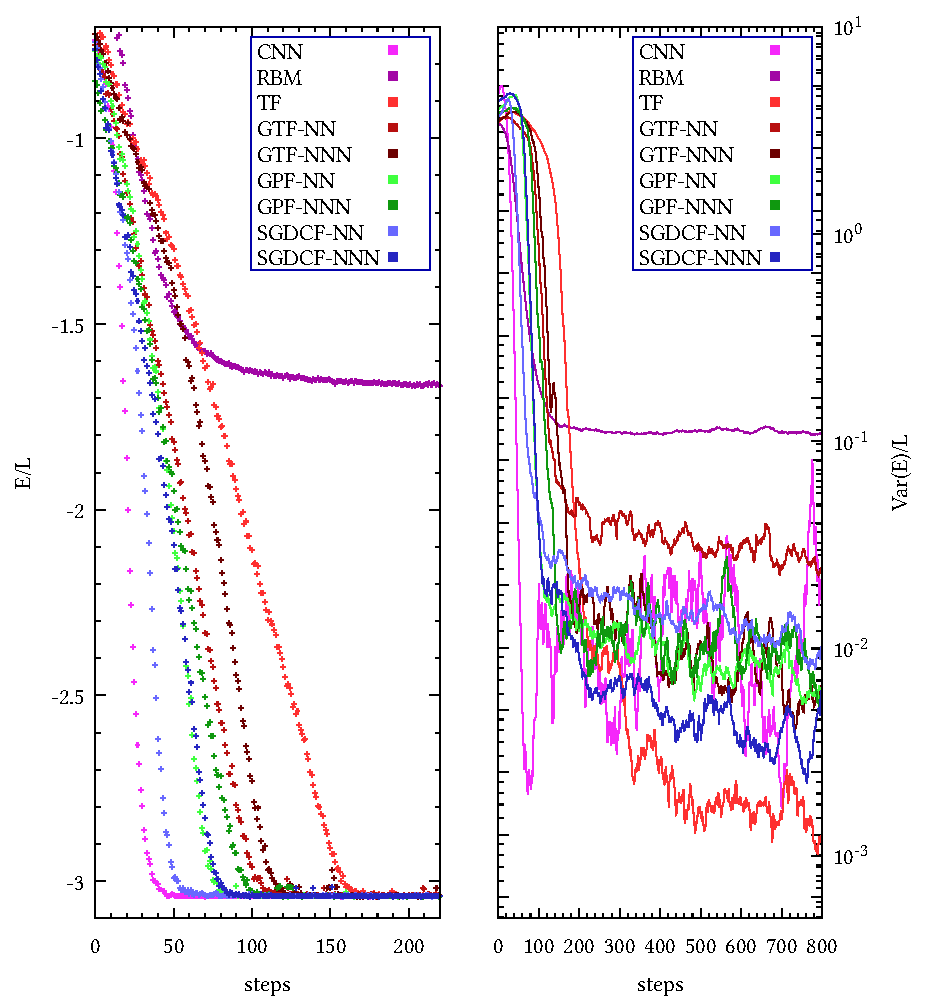
\includegraphics[width=1.1\textwidth]{./experiments/ground-state-search/comparison-established/architecture-comparison/architecture-comparison.pdf}}
    \caption{A comparison of different established and novel neural network architectures used as NQS in a ground state search.
        The calculations were performed for a 2D-trigonal\_hexagonal lattice of size 3 (37 lattice sites).
        The lattice is periodic and the encoding is set to be random.
        The models were configured to be as similar as possible in terms of the number of trainable weights.
        The \emph{CNN} was set to have 16 channels ($\stackrel{\wedge}{=}$ 592 weights), The \emph{RBM} was set have 8 hidden layers ($\stackrel{\wedge}{=}$ 592 weights). 
        All metaformers were set to a depth of 2, and a mlp-ratio of 2.
        The poolformers have an embed-dimension of 7 ($\stackrel{\wedge}{=}$ 560 weights for \emph{GPF-NN} and 602 for \emph{GPF-NNN}).
        The conformers also have their embed dimension set to 7 ($\stackrel{\wedge}{=}$ 602 weights for \emph{SGDCF-NN} and 644 for \emph{SGDCF-NNN}).
        Finally the transformers are set to have an embed-dimension of 5 ($\stackrel{\wedge}{=}$ 530 weights for \emph{TF}, 566 weights for \emph{GTF-NN} and 596 weights for \emph{GTF-NN}). 
        Important to notice are the different scales of the x-axes, the energy per site is only shown until step 200, because after that nothing of interest happens. The variance of the energy is shown until step 800.  
        The variance data is interpolated with a moving average in the logarithmic scale of width 35 steps.
    }
    \label{fig:gss-architectures-comp}
\end{figure}

The two most important metrics in the ground state search are the energy $E$ (in the experiments always the energy per lattice site is stated, as to make the graphs independent from the lattice size) and the variance of the energy $\mathrm{Var}(E)$ (also scaled to the number of lattice sites $L$). 
The energy is important, because it shows an easy to understand macroscopic parameter, that even corresponds to the eigenvalue computable with the numeric solution (\autoref{sec:theory-numericalsolution}).
The variance on the other hand is not as tangible, but still a very important metric.
It can only be zero if the wavefunction is an exact eigenstate of the energy operator. 
Furthermore eigenstates that are not the ground state are exponentially less likely the occur.
So the distance of the calculated variance to zero is a direct measure of how good the ground state wavefunction is represented.
It even is an indication, whether the wavefunction is really parametrized properly, or the calculated energy just happens to be the ground state energy by chance.

Looking at \autoref{fig:gss-architectures-comp}, the behavior of different metaformers in a specific Ising problem can be observed.
The metaformers are compared against a \emph{CNN} and a \emph{RBM} that are bundled in the \emph{jVMC} package \cite{jVMCgithub}.
The RBM is in this case not able to encode the wavefunction, therefore the calculated energy is different from the rest. 
Also the high variance (notice the log scale) indicates the RBM is not suited for representing this wavefunction.
To reiterate, this doesn't mean RBMs are bad, as in literature they have been employed successfully numerous times \cite{restrictedBoltzmanMachines}.

The CNN converged the fastest. It also required the least amount of time for the performance of one step.
Therefore it not only produced its results in less steps, but also the fastest.
The metaformers generally were slower to compute, but not by a significant margin. 
Most of the calculations for one step were in the neighborhood of \SIrange[]{2.5}{4}{} times the step time of the CNN.

Though the variance graph shows, that the state representation of the CNN does not converge as good as any of the metaformers'.
The variance data is highly smoothed to make it possible to display and still the CNN's variance fluctuates over multiple orders of magnitude.
Looking at the raw data it is very obvious, that all the metaformers converge to a more stable representation.
It can also be noted, that by step 800 all of the metaformers' variances are still on a clear downwards trend, so training them longer would probably result in a static increase in precision.

Only by pinning down the desired metrics, a suited network can be selected. 
While in the experiment, the TF network converged by far the slowest, it also showed the best precision - by about one magnitude - after 800 steps. 
So if fast convergence should be achieved, a different network should be used, than if maximum precision is required.

To finally summarize some other observations: The transformer architectures show a clear trend. 
The more of the attention is masked, the less is the network's performance. 
So GTF-NN has the smallest precision, TF the best. On the flip side, because of the more strict inductive bias, the GTF-NN converges the fastest, beating GTF-NNN and TF.

The graph-conformers and poolformers fall into the middle field with similar behavior in regards to the number of interactions.
